%!TEX root = constraint-layout.tex

% \newcommand{\teaserFigure}{
% 	\teaser{
% 		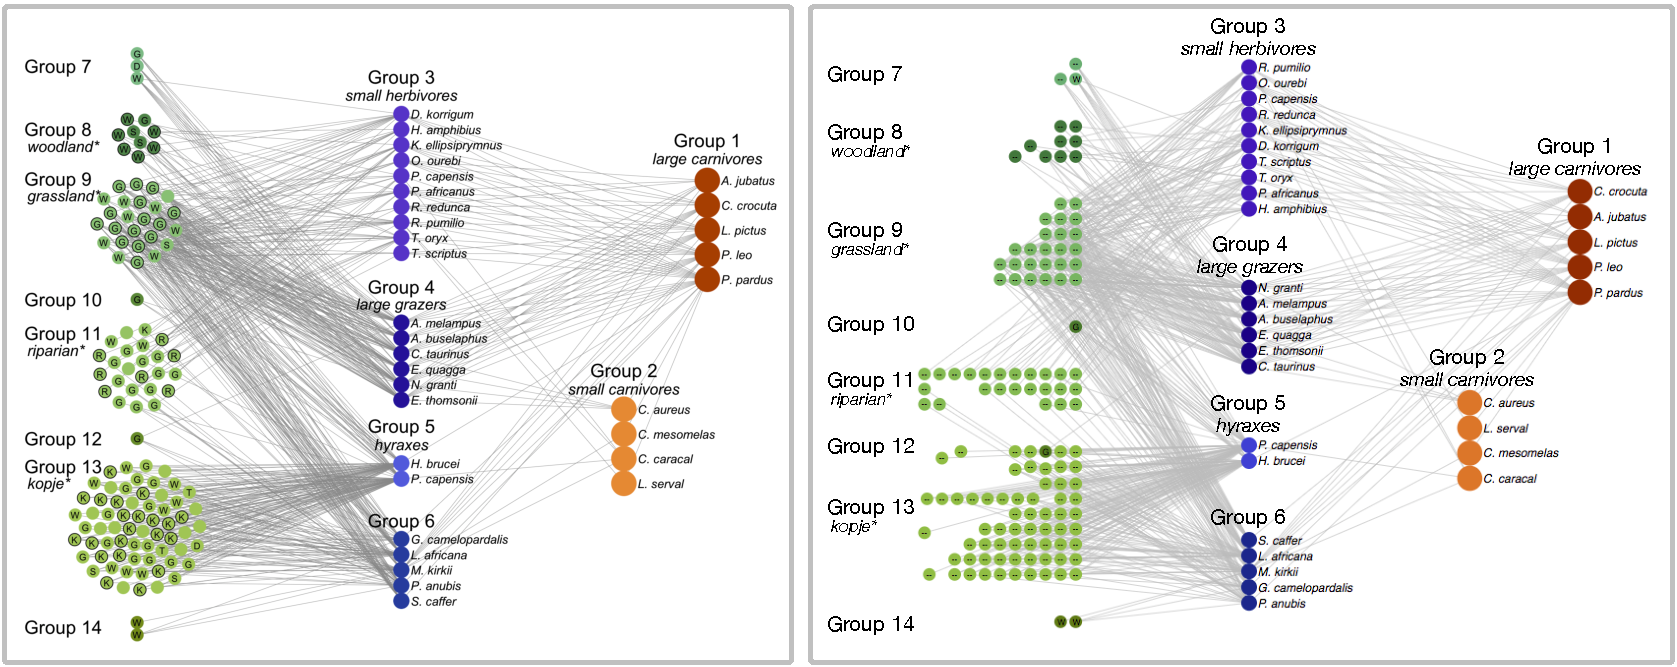
\includegraphics[width=\linewidth]{figures/serengeti-layout.pdf}
% 		\centering
% 	  \caption{\label{fig:teaser}}

% 	}
% }

\newcommand{\serengetiLayoutColumn}{
  \begin{figure}[t!]
    \centering
    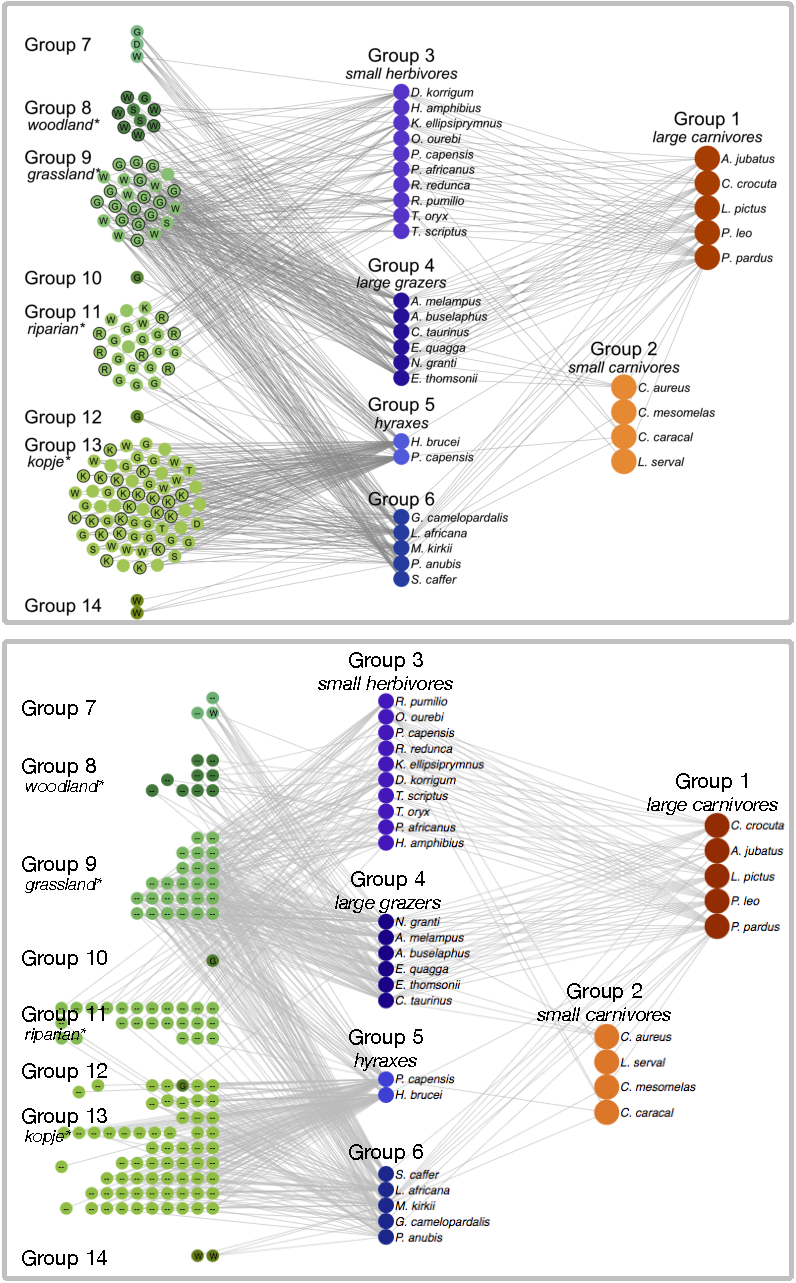
\includegraphics[width=0.81\columnwidth]{figures/serengeti-layout-column.pdf}
    {\caption{\label{fig:serengeti-layout}
    The layout for the Serengeti food web using our constraint language, as compared to Baskerville et al.~\cite{baskerville2011spatial}.}}
    \vspace{-40px}
  \end{figure}
}

%%%%%%%%%%%%%%%%%%%%%%%%%%%%%%%%%%
%%%%%%%%%%%%% Design %%%%%%%%%%%%%
%%%%%%%%%%%%%%%%%%%%%%%%%%%%%%%%%%

\newcommand{\smallTreeExample}{
  \begin{figure}[t!]
    \centering
    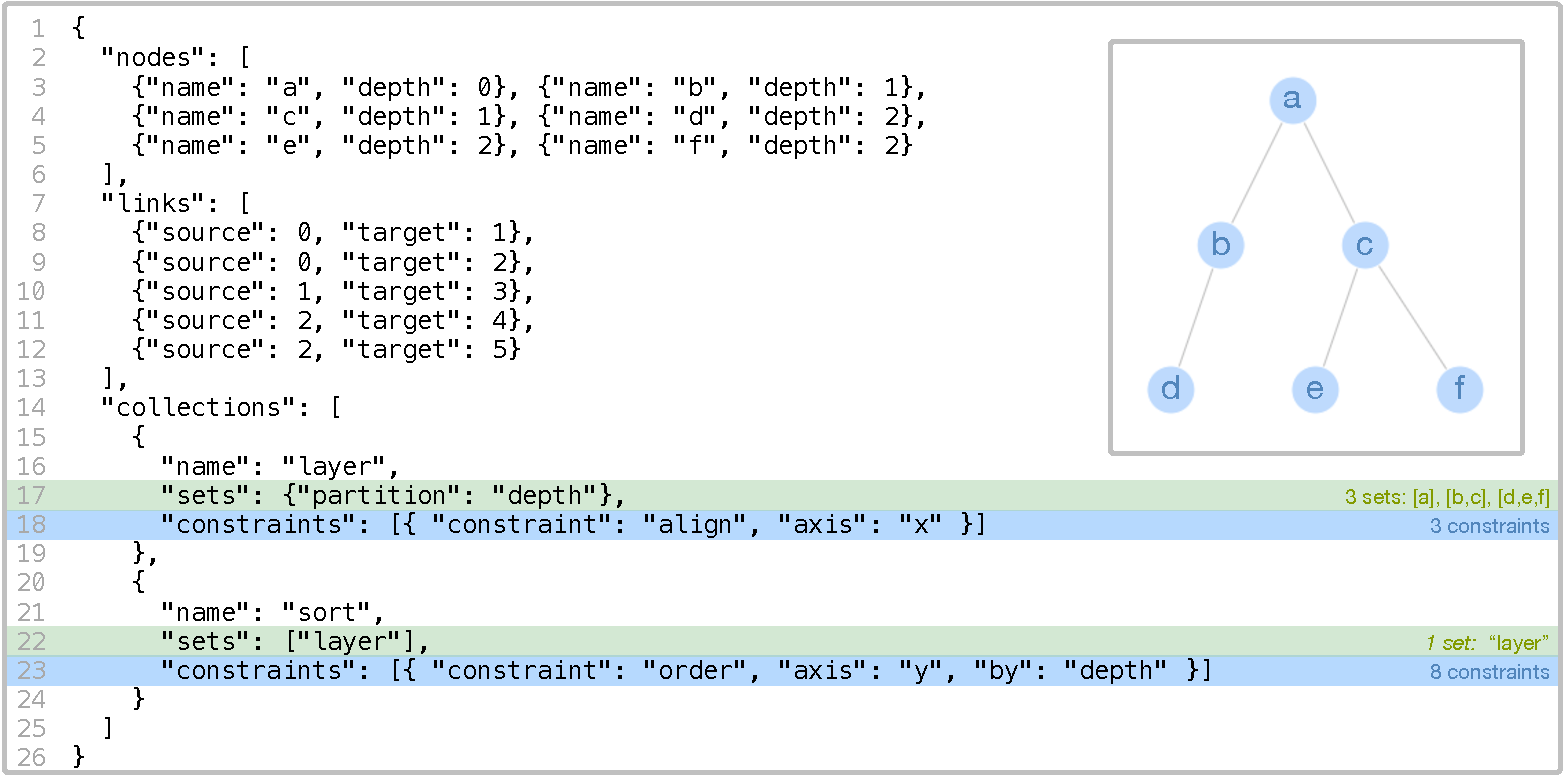
\includegraphics[width=\columnwidth]{figures/small-tree-example.pdf}
      {\caption{\label{fig:small-tree-example} The \projectname specification
      and data for a small tree with six nodes. Nodes are split into sets 
      based on their \texttt{depth} from the root ``\texttt{a}'', and aligned. 
      A new set definition uses composition to include the ``layer'' set
      and the layers are ordered by their depth to form the tree. 
      \feedback{Matt}{Just an idea but maybe write the spec Figure 2. in 
     YAML instead of JSON so its easier to read? Makes your work look better 
     too if the spec looks simpler.} }}
    \vspace{-20px}
  \end{figure}
}

\newcommand{\contradictionExample}{
  \begin{figure}[t!]
    \centering
    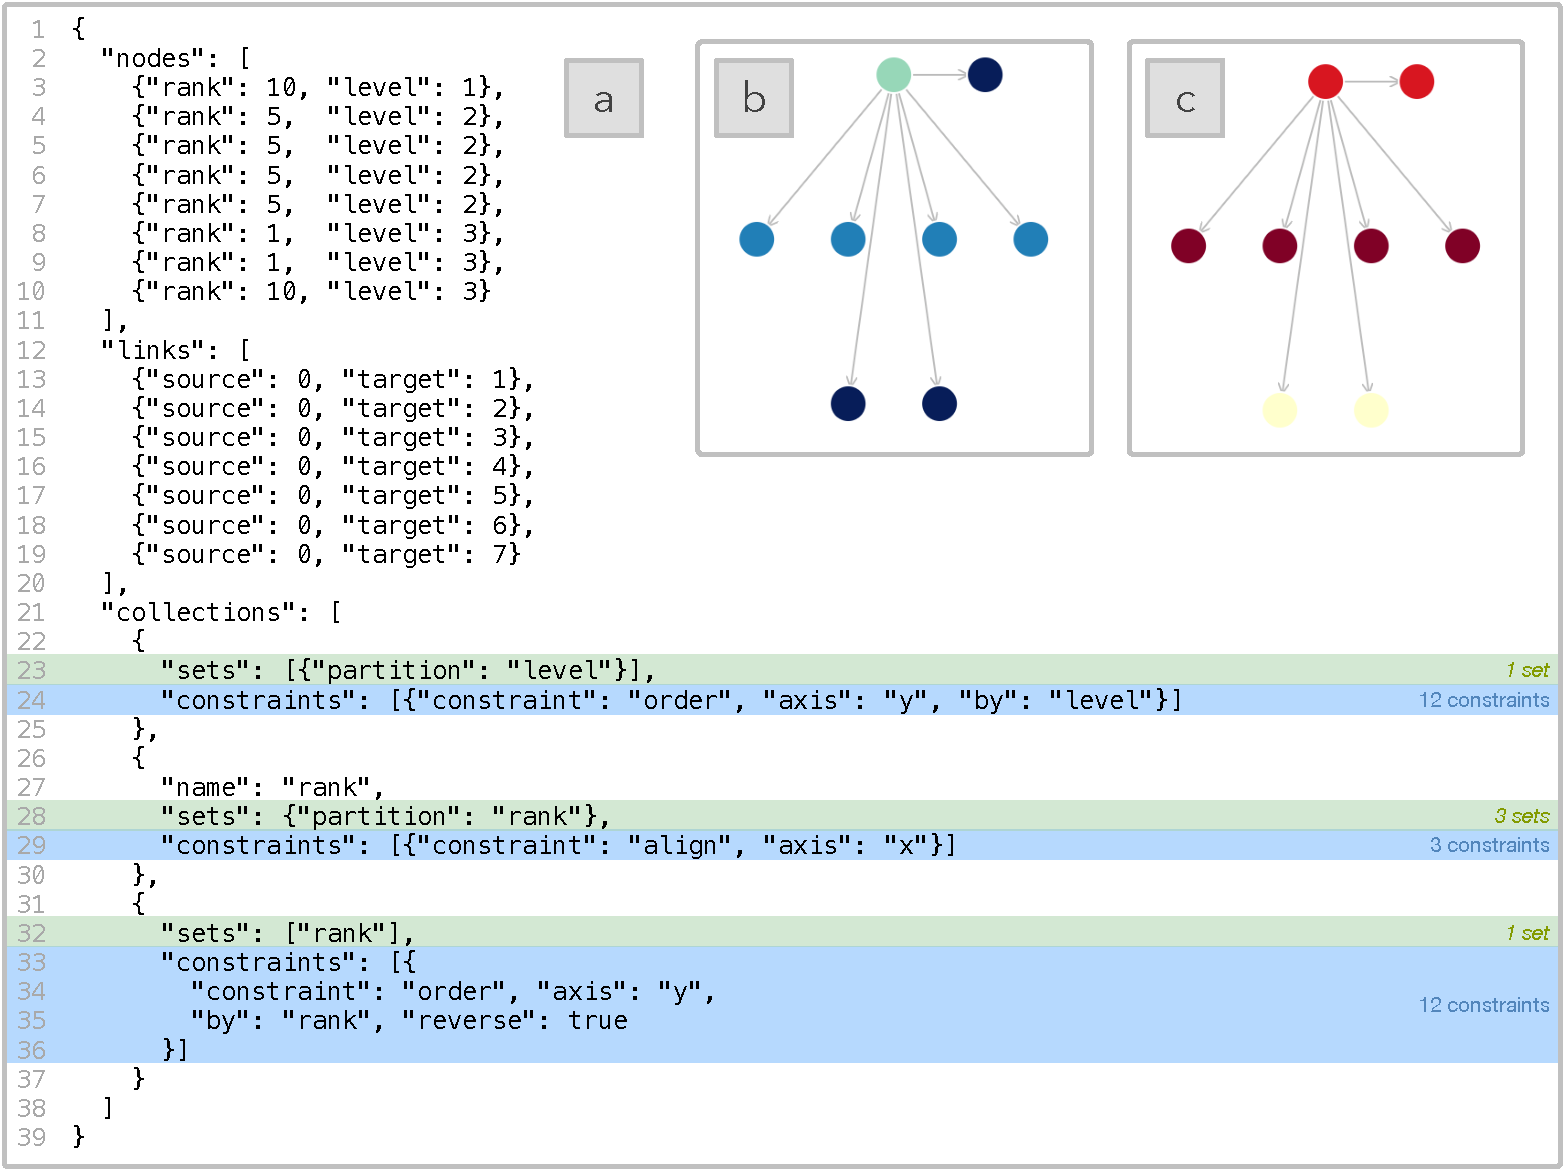
\includegraphics[width=\columnwidth]{figures/contradiction-example.pdf}
                    {\caption{\label{fig:contradiction-example} (a) The
                        full \projectname\ specification for a small graph
                        with eight nodes. (b) Nodes are aligned based on
                        their \texttt{rank}, and colored based on their
                        \texttt{level}. Two constraints are applied to
                        order the nodes, once by \texttt{level} and once by
                        \texttt{rank}, which produces a contradiction. (c)
                        Nodes are colored based on the amount of error for
                        constraints that are invalid.  }}
    \vspace{-20px}
  \end{figure}
}

%%%%%%%%%%%%%%%%%%%%%%%%%%%%%%%%%%
%%%%%%%%% Demonstration %%%%%%%%%%
%%%%%%%%%%%%%%%%%%%%%%%%%%%%%%%%%%

\newcommand{\krugerLayout}{
  \begin{figure}[t!]
    \centering
    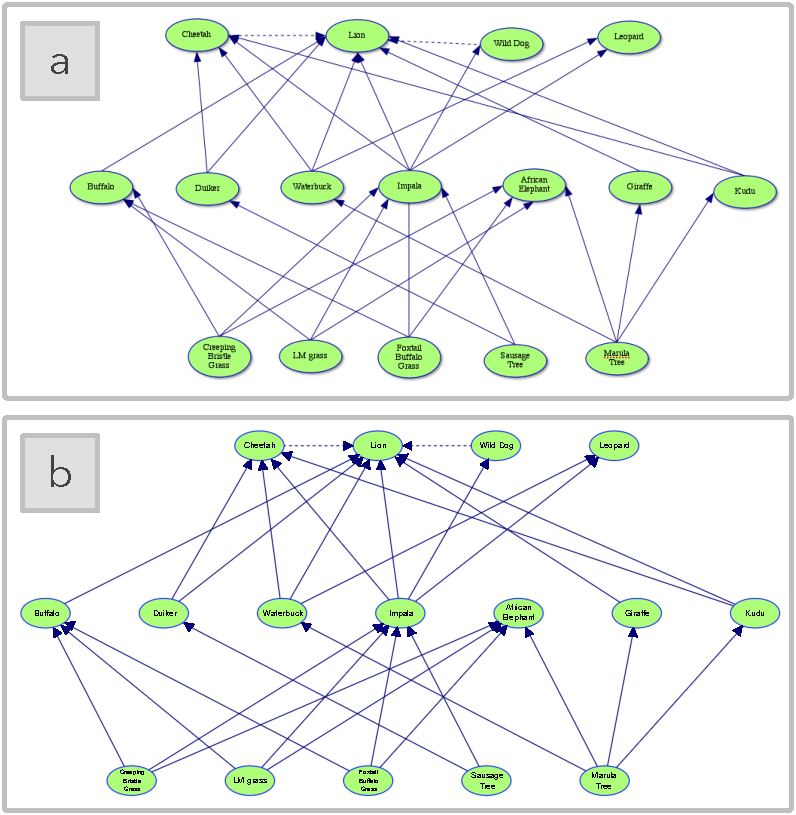
\includegraphics[width=\columnwidth]{figures/kruger-layout.pdf}
    {\caption{
      \label{fig:kruger-layout} A subset of the food web for Kruger 
      National park arranged by trophic level (i.e., carnivore, 
      herbivore, and plant), as seen on the website \cite{kruger2017} 
      and (b) recreated using \projectname. \feedback{Zening}{The (a) and 
      (b) labels in Fig 3, 6, 7 seem a bit large compared to the nodes 
      in the figures and the text font in the paper.}
    }}
    \vspace{-20px}
  \end{figure}
}

\newcommand{\serengetiLayout}{
  \begin{figure*}[t]
    \centering
    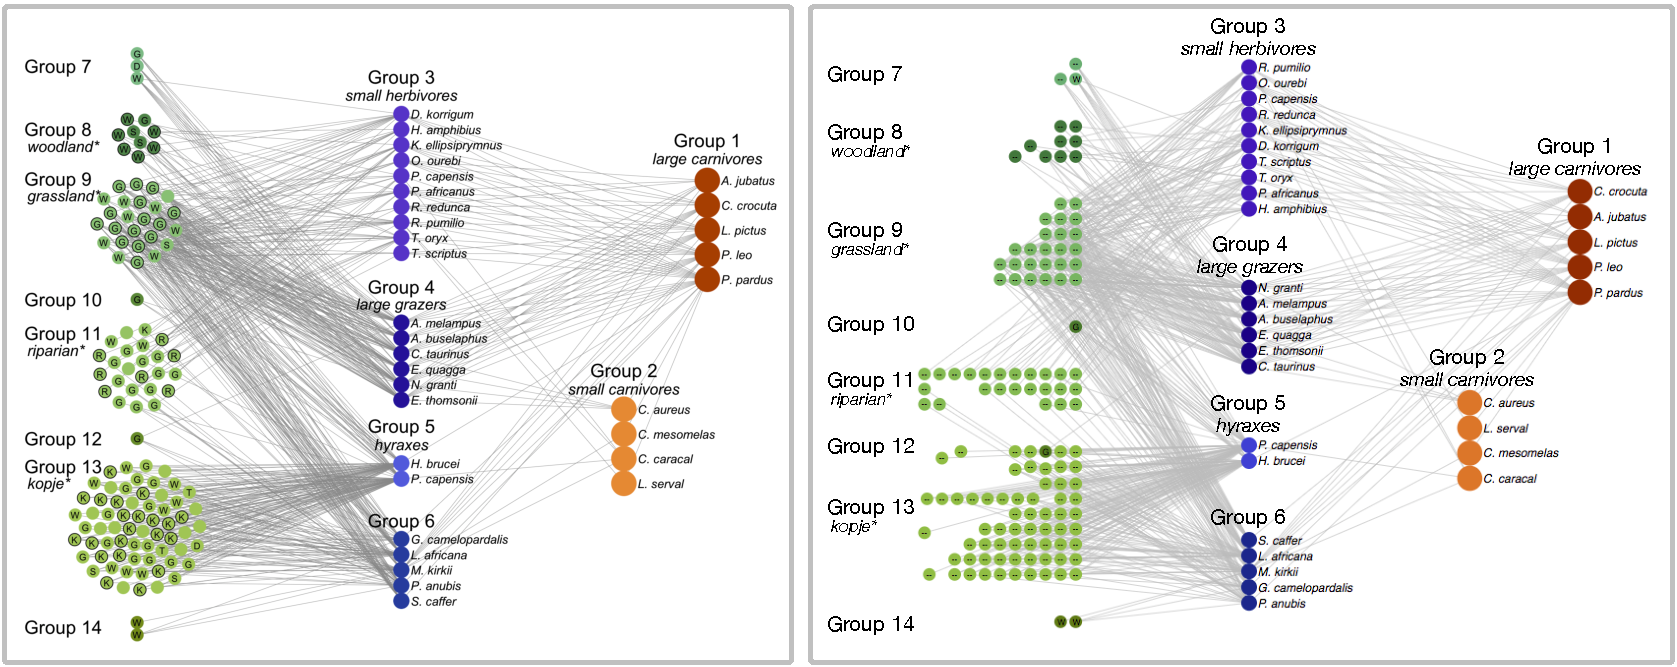
\includegraphics[width=\textwidth]{figures/serengeti-layout.pdf}
    \vspace{-20px} {\caption{\label{fig:serengeti-layout} The layout for
        the Serengeti food web from (a) Baskerville et al.~\cite{baskerville2011spatial}
        as compared to (b) the layout recreated with \projectname.}}
  \end{figure*}
}

\newcommand{\serengetiSpec}{
  \begin{figure}[h!]
    \centering
    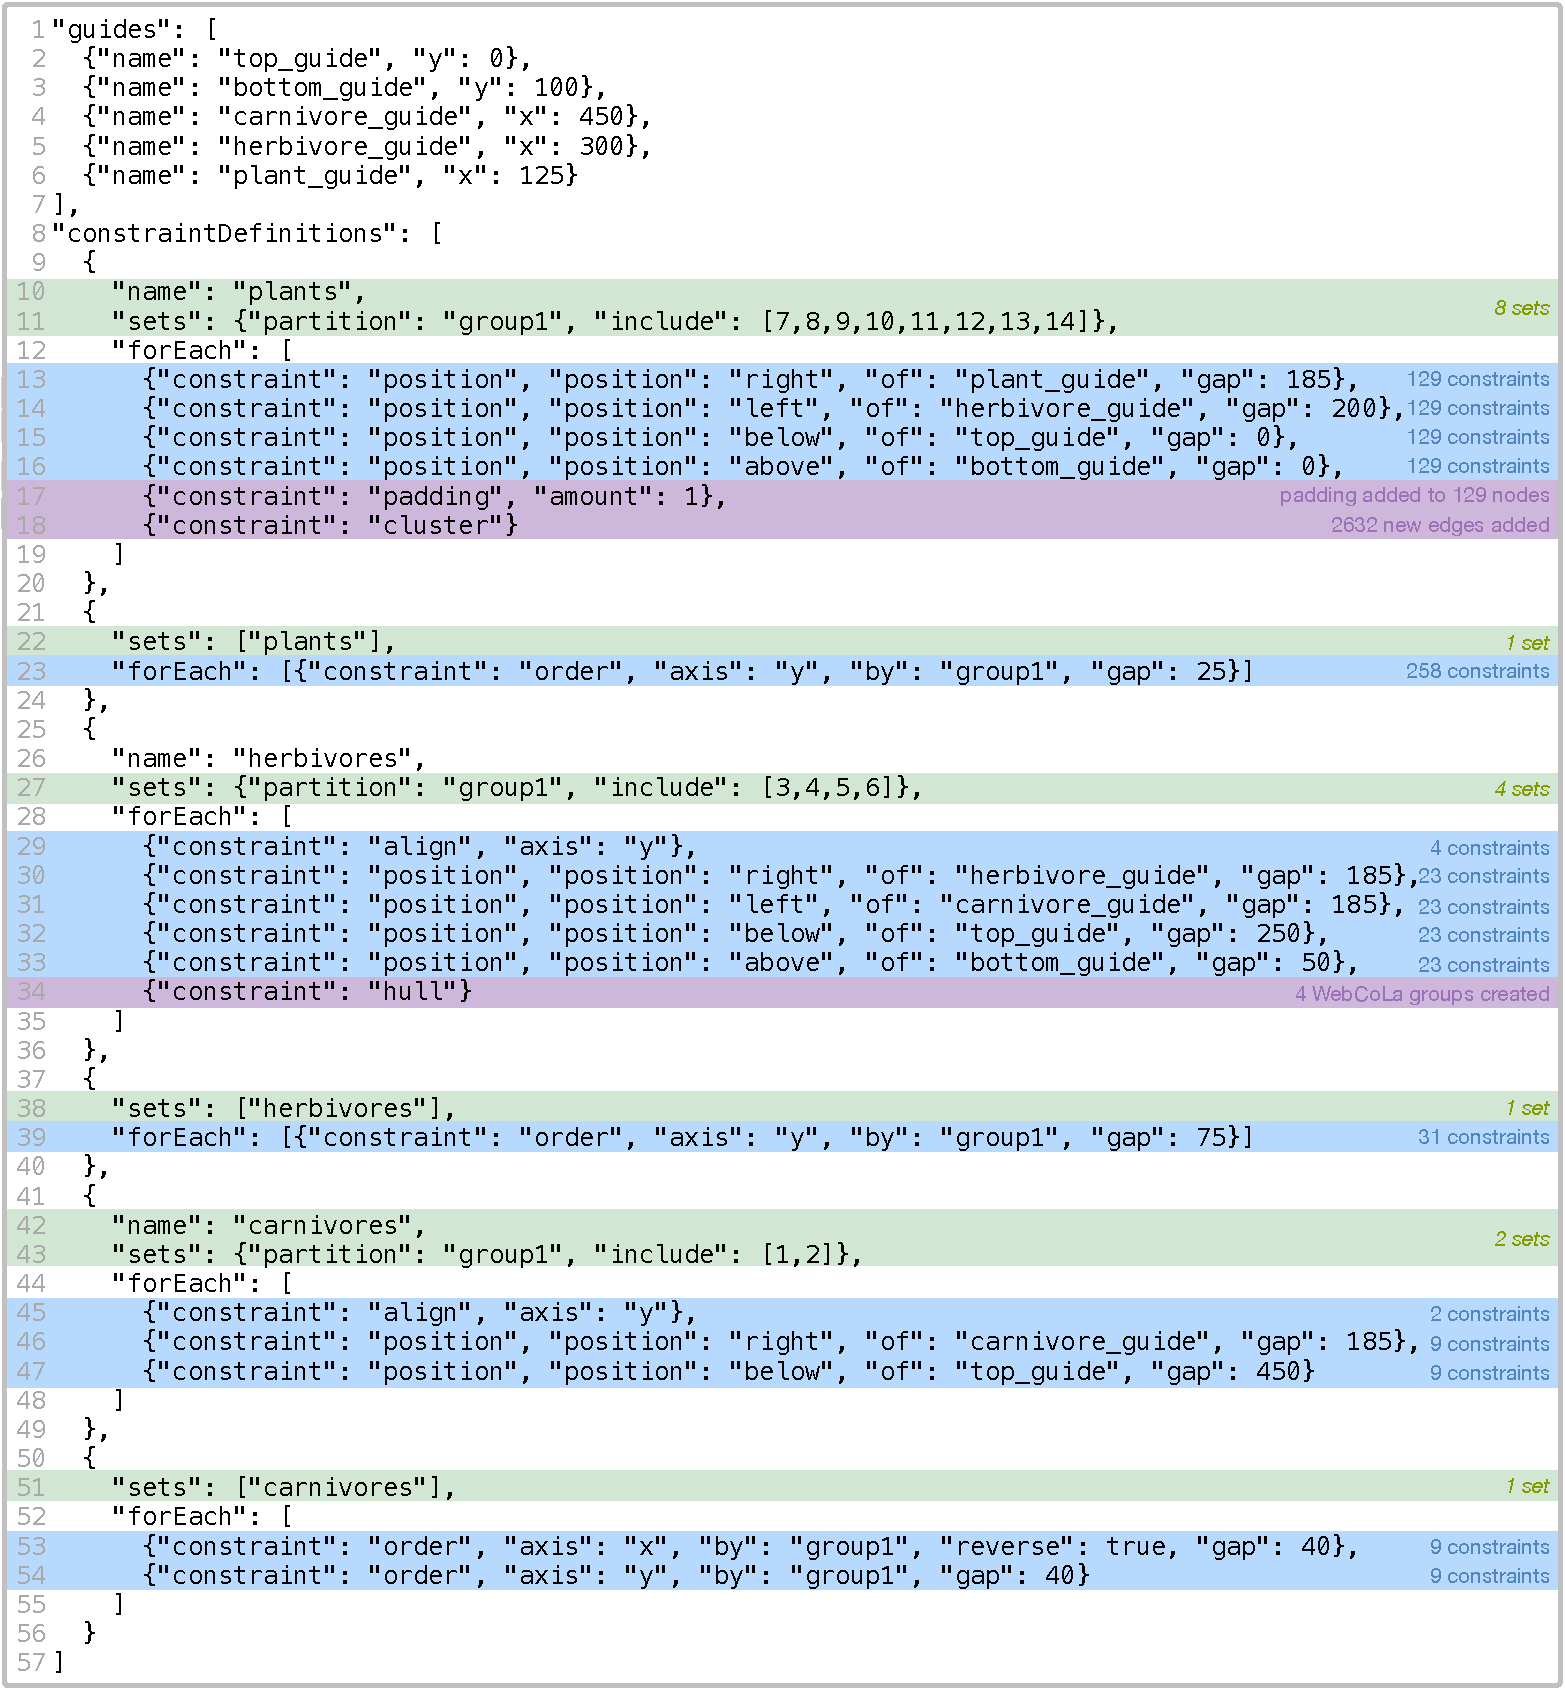
\includegraphics[width=\columnwidth]{figures/serengeti-spec.pdf}
    \vspace{-20px} {\caption{\label{fig:serengeti-spec} The
        \projectname~specification for the Serengeti food web shown in
        Figure~\ref{fig:serengeti-layout}. The code is annotated with the
        number of sets produced, the number of edges added, and the number
        of WebCoLa constraints generated for the final layout.}}
    \vspace{-10px}
  \end{figure}
}

\newcommand{\syphilisLayout}{
  \begin{figure*}[t]
    \centering
    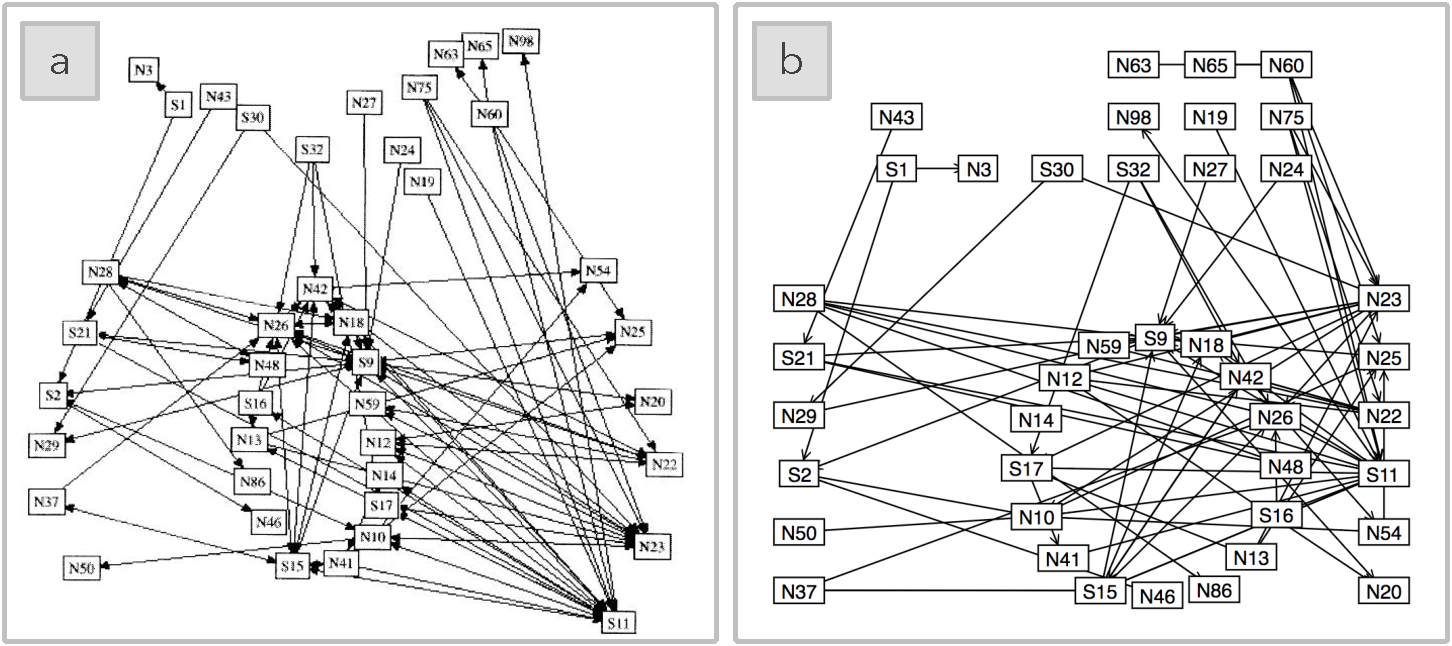
\includegraphics[width=\textwidth]{figures/syphilis-layout.pdf}
    \vspace{-20px} {\caption{\label{fig:syphilis-layout} The layout for the
        syphilis social network from (a) Rothenberg et
        al.~\cite{rothenberg1998using} as compared to (b) the
        \projectname~layout. \feedback{Zening}{When I first saw this 
        figure and its caption, I wasn't sure if you are just re-creating 
        the original figure or you are improving the original figure. 
        After reading the corresponding text (Sec 5.1), I understand (b) 
        is an improved layout. I think it will be helpful to (briefly but 
        explicitly) say in the caption that b is an improved layout, it 
        makes the ``intensity of interaction'' more clear, as described in 
        the original paper.} \feedback{Zening}{Could you annotate/label 
        the ethnographic groups? Affluent white men, younger white women, 
        African-American men...}}}
  \end{figure*}
}

\newcommand{\syphilisSpec}{
  \begin{figure}[t]
    \centering
    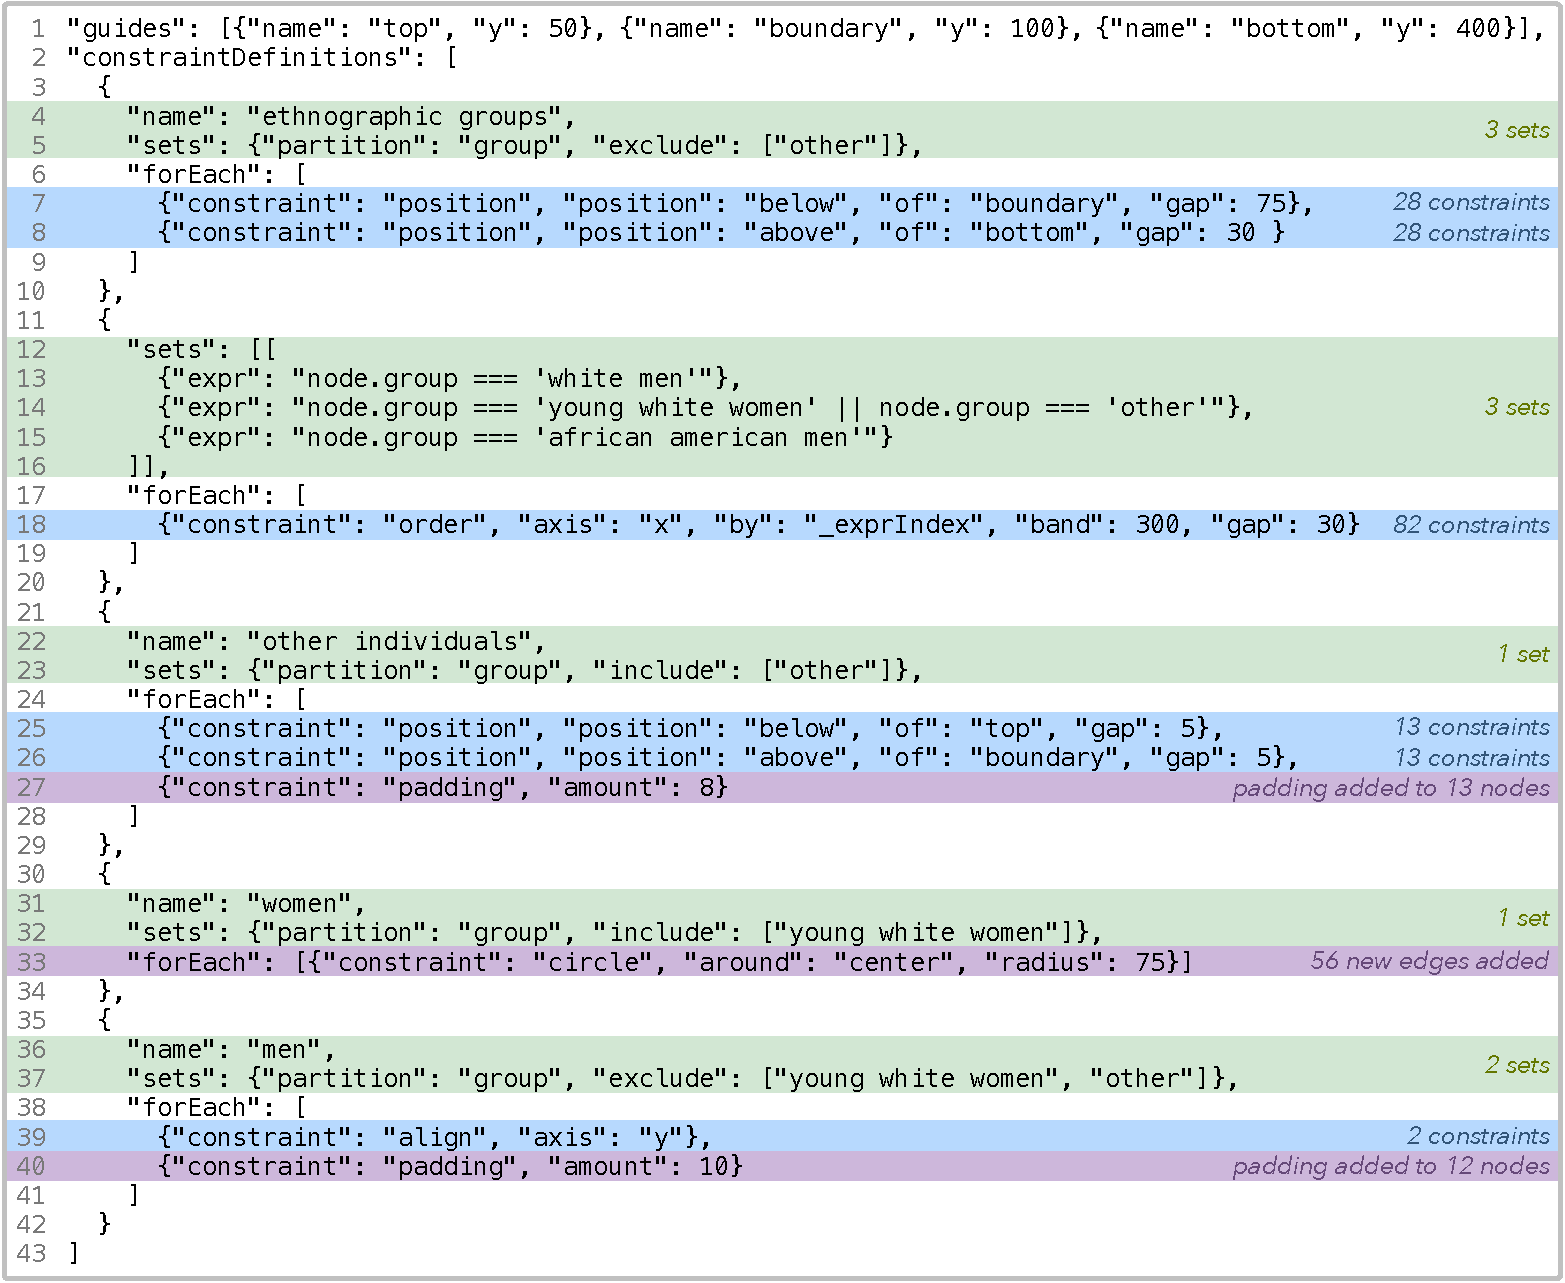
\includegraphics[width=\columnwidth]{figures/syphilis-spec.pdf}
    \vspace{-20px} {\caption{\label{fig:syphilis-spec} The
        \projectname~specification for the syphilis social network shown in
        Figure~\ref{fig:syphilis-layout}. The code is annotated with the
        number of sets produced, the number of edges added, and the number
        of WebCoLa constraints generated for the final layout. 
        \feedback{Zening}{Green annotates the number of sets produced. 
        Blue and purple annotates the number of constraints? Which color 
        annotates the number of edges added? I don't think this need to 
        be repeated in Fig 5 and Fig 8 captions}}}
  \end{figure}
}

\newcommand{\tlrfourLayout}{
  \begin{figure}[t!]
    \centering
    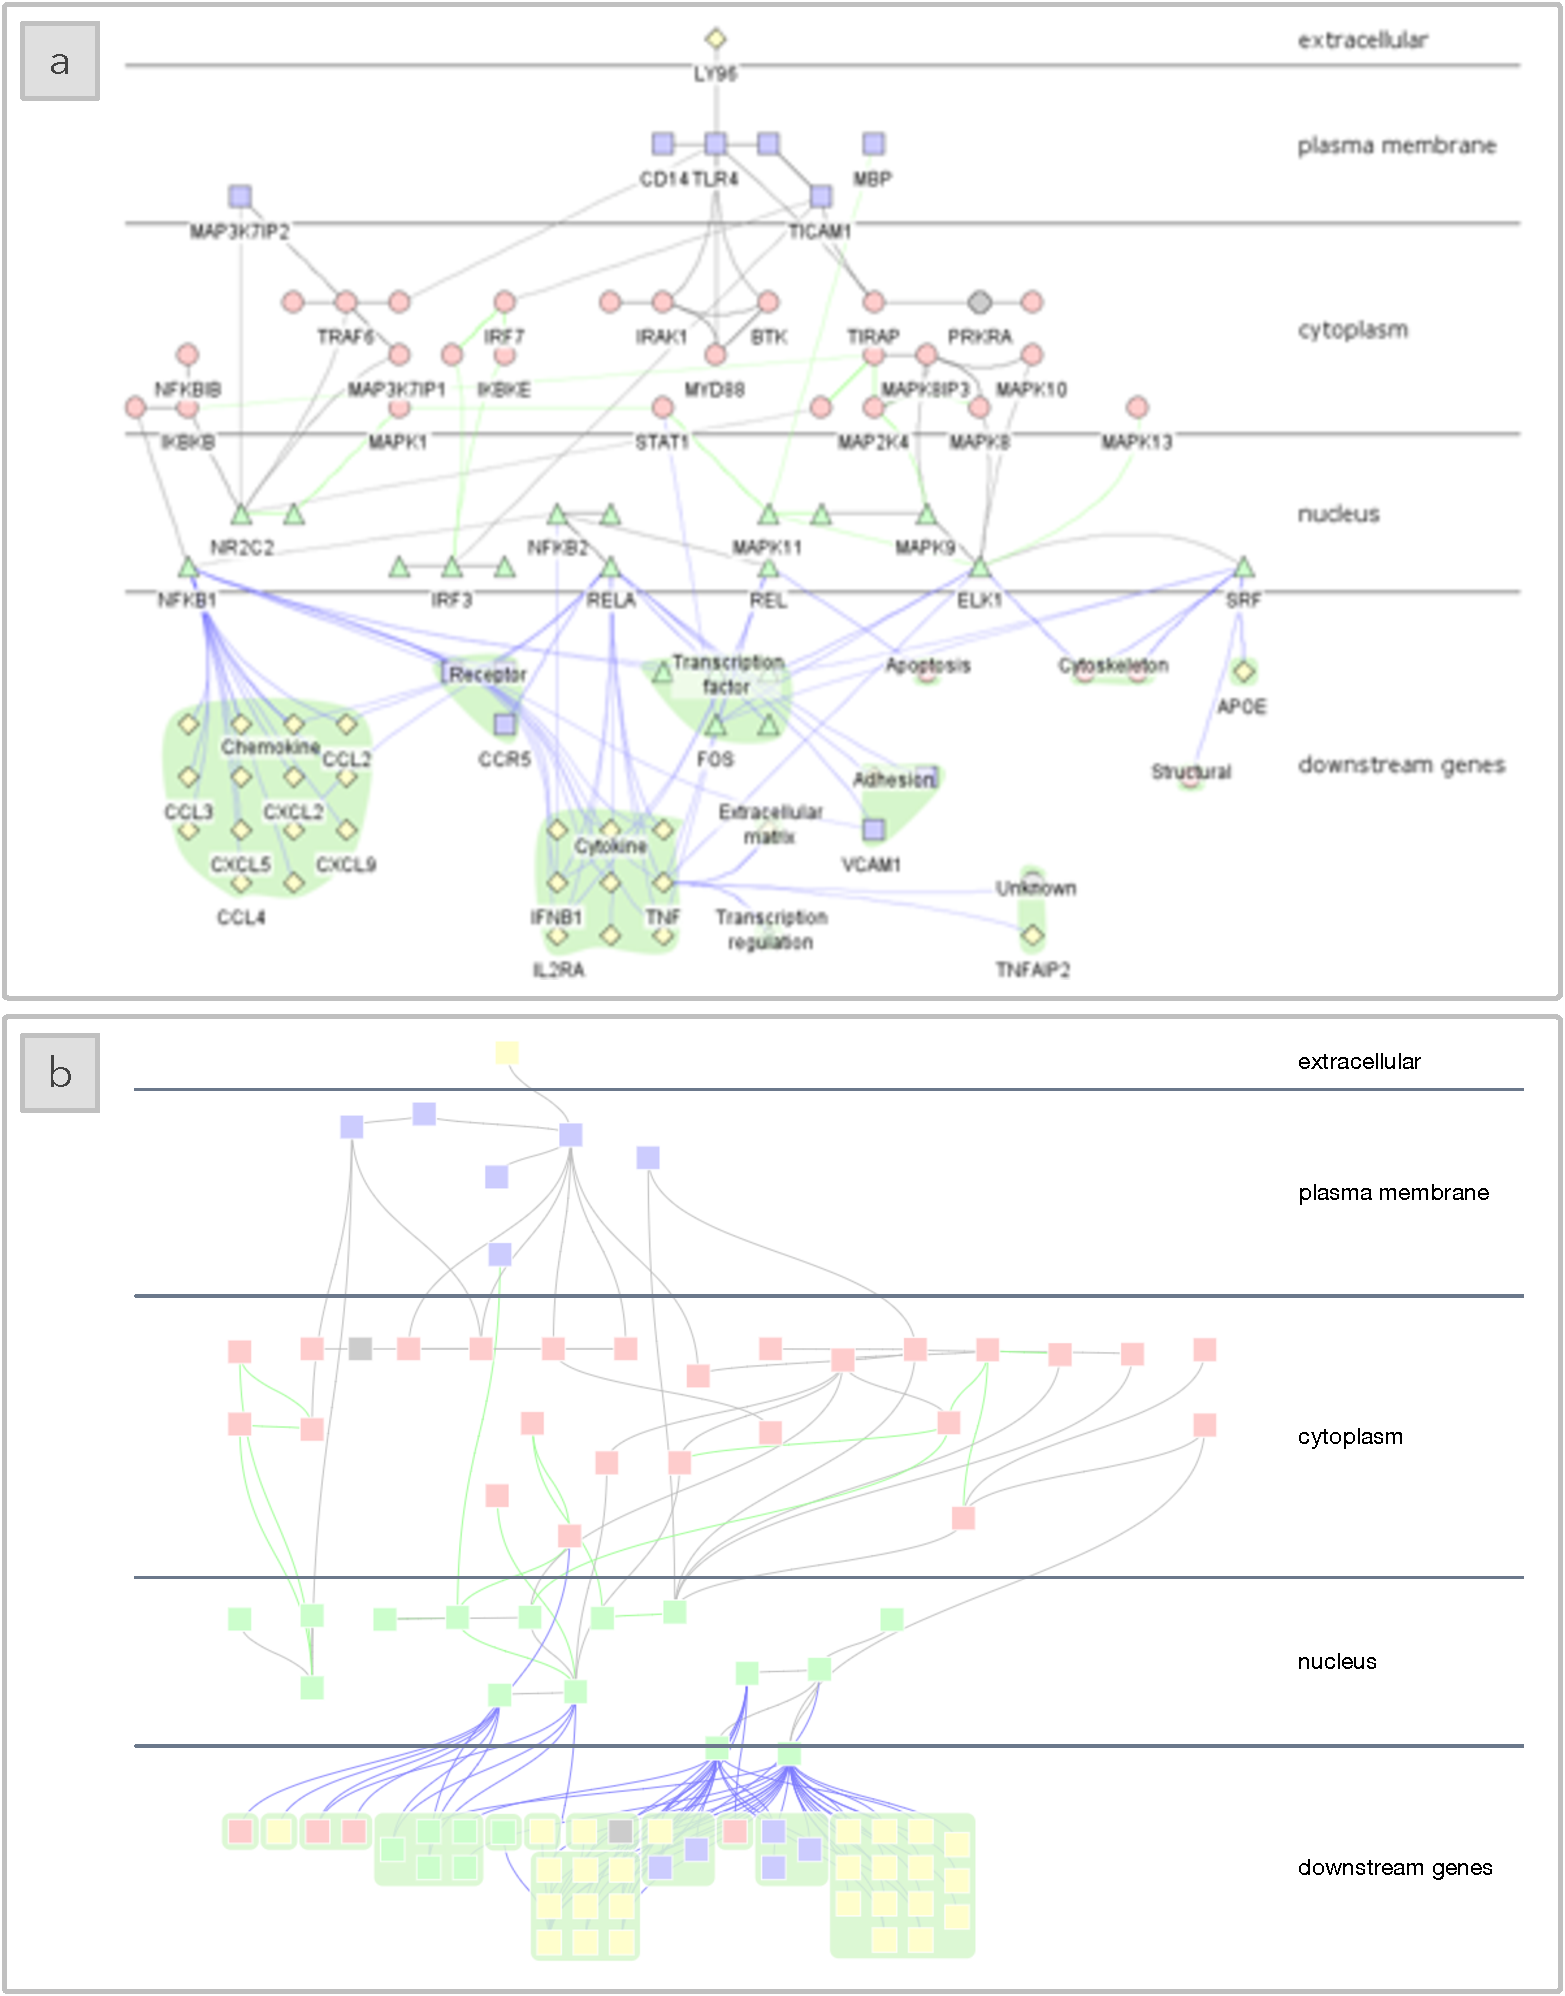
\includegraphics[width=\columnwidth]{figures/tlr4-layout.pdf}
    \vspace{-10px} {\caption{\label{fig:tlr4-layout} The layout for
        the TLR4 biological system produced using (a) Cerebral~\cite{barsky2008cerebral},
        a domain-specific layout tool, as compared to (b) \projectname.
    }}
    \vspace{-30px}
  \end{figure}
}

\newcommand{\tlrfourSpec}{
  \begin{figure}[t]
    \centering
    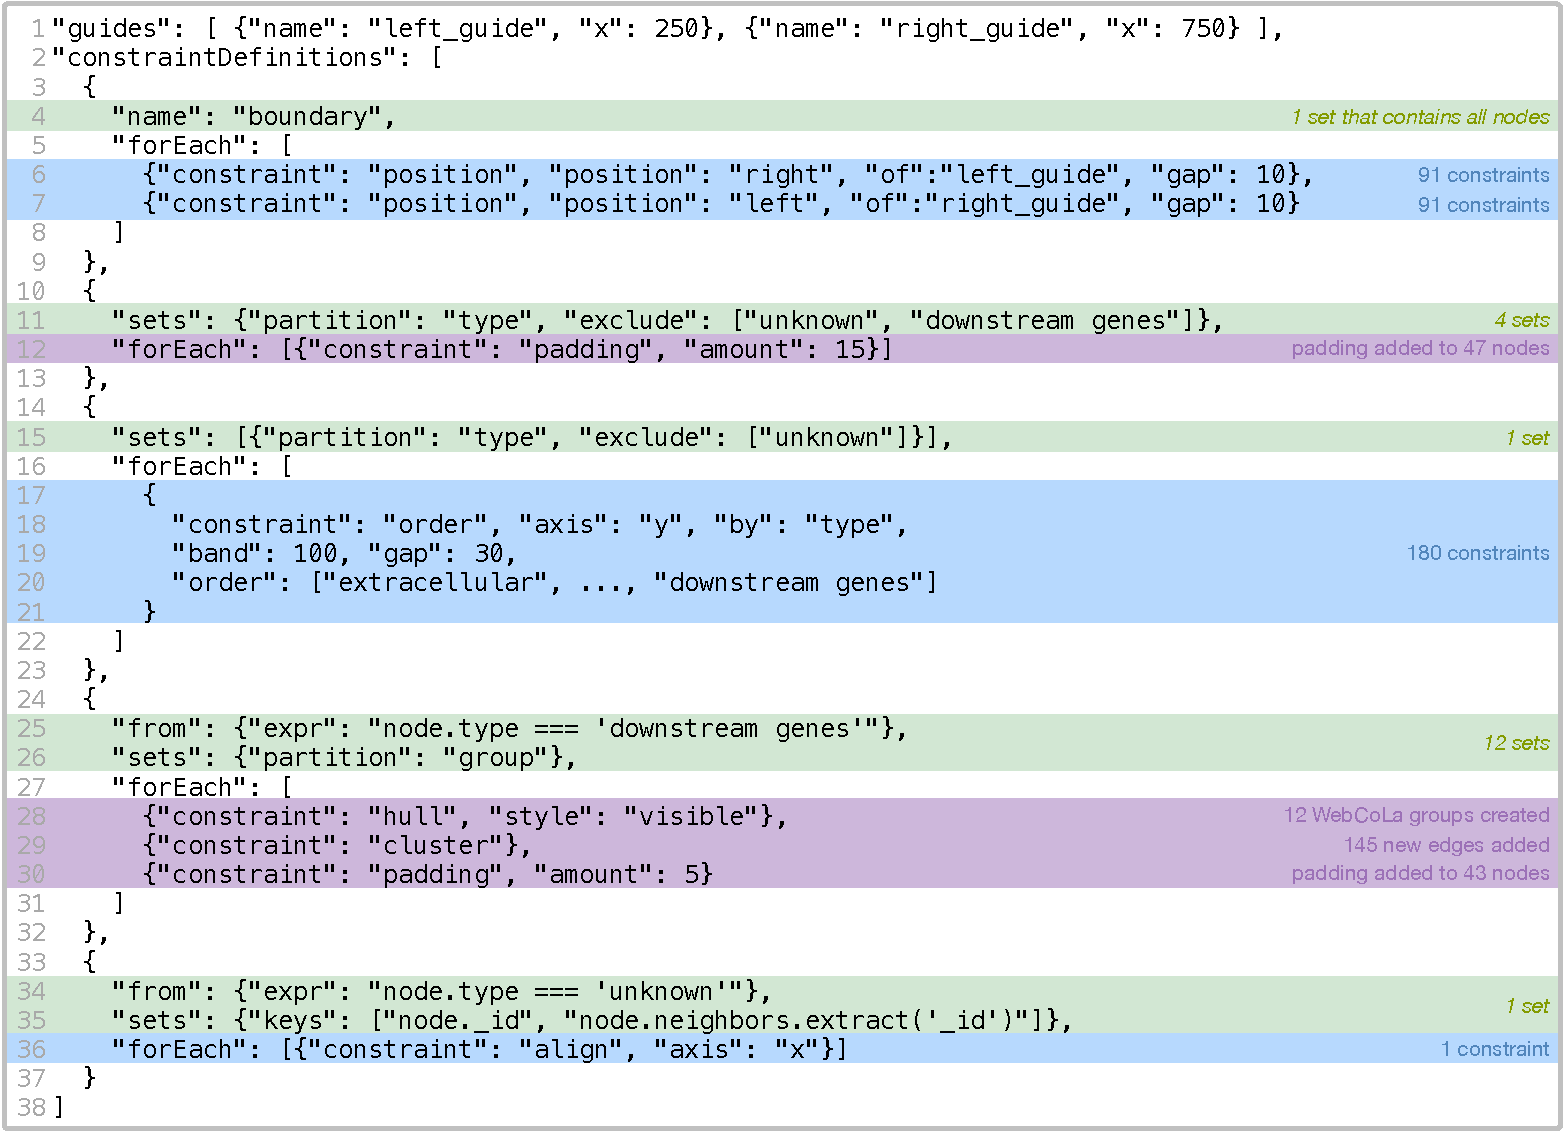
\includegraphics[width=\columnwidth]{figures/tlr4-spec.pdf}
    \vspace{-20px} {\caption{\label{fig:tlr4-spec} The
        \projectname~specification for the TLR4 biological system shown in
        Figure~\ref{fig:tlr4-layout}. The code is annotated with the
        number of sets produced, the number of edges added, and the number
        of WebCoLa constraints generated for the final layout.
        \feedback{Younghoon}{I could infer what ``from'' and ``forEach'' 
        mean in TLR4. But hard to infer ``collect''. (I might miss the 
        description for these...).}}}
  \end{figure}
}

\newcommand{\constraintsFigure}{
  \begin{figure}[t]
    \centering
    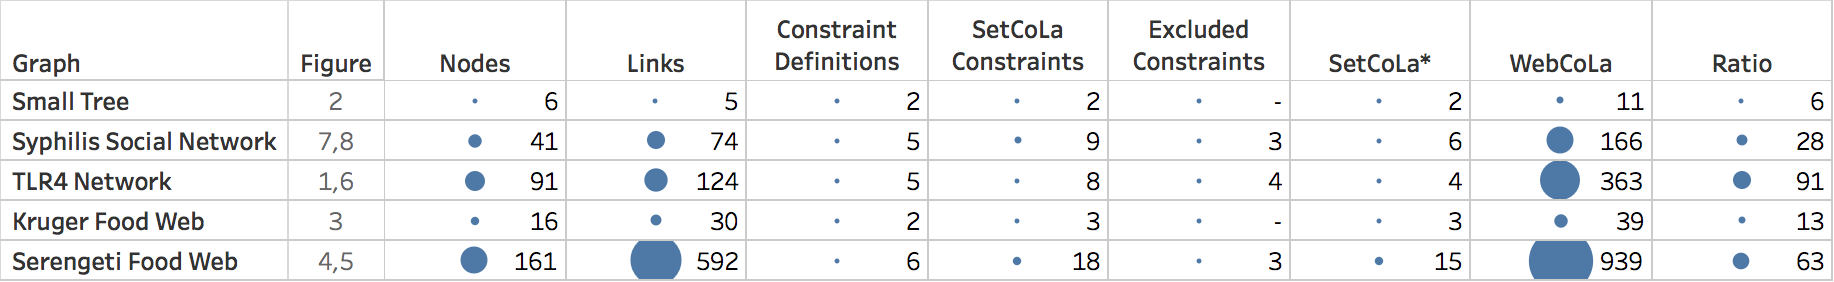
\includegraphics[width=\columnwidth]{figures/constraints.png}
    \vspace{-20px} {\caption{\label{fig:constraints}
    The number of nodes, links, and constraints for each example. We show
    the number of constraint definitions and number of SetCoLa constraints
    written by the user as well as the number of WebCoLa constraints
    generated by the compiler. \todo{some SetCoLa constraints are not 
    translated to WebCoLa constraints, so the comparison is a bit off...}
    \feedback{Matt}{Figure 9 is great. Put that earlier / make it more prominent?
    (also maybe edit so the numbers don't overlap the circles)}
    \feedback{Zening}{In Fig 9, I think the number of constraints in 
    SetCoLa vs. WebCoLa is very impressive. Maybe you could mention that in the abstract.}}}
  \end{figure}
}